Similar to the construction of the algorithm in the last section, \citet{agmw07} show that the contact map overlap between a $2$-stack and any two dimensional graph can be constructed in $O({n_1}{n_2}^{2}\log n_1)$ time where $n_1$ is the number of vertices in the $2$-stack and $n_2$ is the number of vertices in the two dimensional graph. To illustrate the same, the stack has been represented as a tree where each node corresponds to an edge of the tree and a node $e^{\prime}$ can be considered as the child node of $e$ when $e$ contains $e^{\prime}$ \citep{agmw07}.

\begin{figure}[htbp]
\begin{minipage}[b]{0.5\linewidth}
\centering
 
\centering
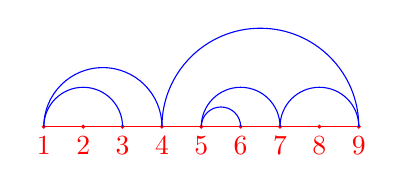
\begin{tikzpicture}[scale=0.5]


\foreach \i in {1,...,8} {
        \draw[red] (\i,1) -- (\i + 1,1)node[pos=0.0,below] {\i};
        \filldraw[red] (\i,1) circle (1pt);


 }

\draw[red] (9,1) -- (8,1)node[pos=0.0,below] {9};
\filldraw[red] (9,1) circle (1pt); 



\draw[blue, thin] (1,1) arc(180:0:1); 
\draw[blue, thin] (1,1) arc(180:0:1.5);
\draw[blue, thin] (4,1) arc(180:0:2.5); 
\draw[blue, thin] (5,1) arc(180:0:0.5); 
\draw[blue, thin] (5,1) arc(180:0:1);
\draw[blue, thin] (7,1) arc(180:0:1);

\end{tikzpicture} 
 \vspace{0.65cm}
\end{minipage}
\begin{minipage}[b]{0.5\linewidth}
\centering
 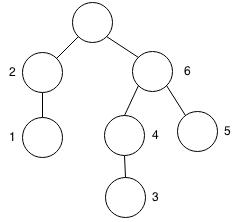
\includegraphics[width=0.5\textwidth]{tree}
 \vspace{0.65cm}
\end{minipage}
\caption{Stack and its tree representation}
 \label{fig:stacktree}
\end{figure}
The authors show the results for a $1$-stack and any two dimensional graph and then the results are extended to compute the overlap between a $2$-stack and graph. Let
$G_1 = (V_1,E_1)$ be the 1-stack of size $n_1$ and $G_2 = (V_2,E_2)$ a contact map of size $n_2$. Further, let $e \in E_1$ be the rightmost edge in $G_1$ with the highest right end-point and $e^{\prime} \in E_2$ be a similar edge in $G_2$. Since $G_1$ is a 1-stack, $e$ is not contained in any other edge, so $e$ and $e^{\prime}$ must match each other. If $(v_l,v_j)$ be the end points of such an edge $e$ in $G_1$ and $(v_{l^{\prime}},v_{j^{\prime}})$ be the edge of $e^{\prime}$ in $G_2$, then the problem can be divided into two subproblems where $(v_i,v_l)$ and $(v_l,v_j)$ are the starting and ending vertices of the two subgraphs of $G_1$, and $(v_{i^{\prime}},v_{l^{\prime}})$ and $(v_{l^{\prime}},v_{j^{\prime}})$ are the starting and ending vertices of the two subgraphs of $G_2$. Hence, the maximum contact overlap can be computed by the same dynamic programming technique used by \citet{goip99} where at each step the graph is divided into subgraphs with respect to the rightmost edge. Thus the quantity $D(i,j,i^{\prime},j^{\prime})$, the optimal match between $v_i,\cdots,v_j$ and $v^{\prime}_i,\cdots,v^{\prime}_j$, can be given by:
\begin{equation}
\label{scmo1}
D(i,j,i^{\prime},j^{\prime}) = \max\{D(i,j-1,i^{\prime},j^{\prime}),D(i,j,i^{\prime},j^{\prime}-1),(D(i,l-1,i^{\prime},l^{\prime}-1)
+D(l,j-1,l^{\prime},j^{\prime}-1)+1)\},
\end{equation}
where $(v_l,v_j) \in E_1$ and $(v^{\prime}_l,v^{\prime}_j) \in E_2$. The time taken to compute this is $O({n_1}^2{n_2}^2)$. In the equation, the last 1 is when the rightmost edge of each have been mapped. This is known as the ``right matching" algorithm. Similarly the algorithm which matches the left edges is known as the ``left matching" algorithm, the running time of which is still $O({n_2}^4)$. Using a tree decomposition theorem proposed by \citet{klein98}, \citet{agmw07} show that if the process is interleaved, \emph{i.e.} at some points the rightmost edges are matched and at others the leftmost edges are matched thereby meeting in the middle, then the total number of edges that need to be visited is $O({n_1} \log {n_1})$. This is where the tree structure of the stack becomes useful. These edges need to be mapped to all the edges of $V_2$ requiring $O({n_2}^2)$ time. Hence, the total time to compute $D$ is $O({n_1}{n_2}^2\log n_1)$. The vertices which have degree 2 are also handled in the same time bound.

\citet{goip99} show that any two-dimensional contact map can be decomposed into two 2-stacks and two 2-staircase. Further, each 2-staircase can be decomposed into two 1-staircase in linear time. Considering two-dimensional contact maps $G_1$ and $G_2$ of size $n$ each, $G_1$ can be decomposed into six subgraphs and then maximum contact overlap can be calculated between the set of these $6$ subgraphs and $G_2$ rendering a 6-approximation algorithm. The maximum time taken is $O(n^3\log n)$. 